\scanpage{74}
\mspage{73}

\handwritten{7.} We shall see above that the answer to the preceding question is affirmative when $k$ is a finite field, in particular if it is the prime \unsure{coops|field} $\underline{F}_p$, One then finds, thanks to this extension structure on $\underline{G}(\underline{F}_p)$, a canonical homomorphism of Gerbes (for every $k$)
\[
\underline{G}(k)\handwritten{\simeq}\underline{G}(\underline{F}_p)\mathrm{x}_{\deleted{\unsure{\underline{G}(}}\handwritten{\unsure{\underline{\pi}|\underline{\Pi}}}_p(\underline{F}_p))}\handwritten{\underline{\pi}}_p(k)\ ,
\]
and for $k$ perfect, an affirmative answer to the preceding question amounts to the assertion that the preceding homomorphism is an equivalence of Gerbes. Since one knows perfectly well the Gerbe $\underline{G}(\underline{F}_p)$ and its homomorphism into $\handwritten{\underline{\pi}}_p(\underline{F}_p)$ (cf below) this would therefore give the structure of $\underline{G}(k)$ in terms of the \unsure{connaiasance|knowledge} of \deleted{$\unsure{\pi|\Pi}_p(\underline{F}_p$} $\handwritten{\underline{\unsure{\Pi|\pi}}}_{\deleted{\unsure{a}}p}(k)$ (known when\handwritten{\begin{tikzpicture}[baseline=0cm,x=1cm,y=1cm]\draw[thin] (0,-.45)--(.17,.45);\end{tikzpicture}}one knows $\handwritten{\pi}_1(k)=\operatorname{Gal}(\handwritten{\bar{k}}/k)$) and \deleted{of} the homomorphism $\handwritten{\underline{\pi}}_p(k\deleted{\unsure{Fr|F_p}})\handwritten{\longrightarrow\underline{\pi}}_p(\underline{F}_p)$ (known when one knows $\handwritten{\pi}_1(k)\handwritten{\longrightarrow\pi}_1(\underline{\unsure{\mathbb{F}|\rlap{$K$}F}}_p)\handwritten{\longrightarrow}\handwritten{\hat{\underline{Z}}}$). This would therefore resolve the question of the structure of $\underline{G}(k)$ for $k$ perfect. One will note that the Tate object of $\mathrm{Fc}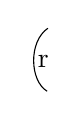
\begin{tikzpicture}[baseline=(r.base),x=1cm,y=1cm]\node[inner sep=0pt] (r) {$\mathrm r$};\draw[thin] (.06,.42)..controls (-.19,.25) and (-.17,-.25)..(.05,-.38);\end{tikzpicture}\mathrm{iso}(k)$ comes from that of $\mathrm{Fcriso}(\underline{F}_p)$ and will therefore also be determined. The canonical fibre functor over $K$\inserted{$=K(k)$}\handwritten{\begin{tikzpicture}[baseline=0cm,x=1cm,y=1cm]\draw[thin] (0,-.3)--(.05,.05)..controls (.1,.16) and (.2,.12)..(.3,.12)--(1.1,.14);\end{tikzpicture}} then corresponds to a fibre functor on $\mathrm{Fcriso}(\underline{F}_p)$ over $K$, a fibre functor on \deleted{$\underline{\unsure{\pi|\Pi}}_p(k)$}\inserted{the categor\unsure{\.{y}|y} of constructible $\underline{Q}_p$-sheaves on $k$}\handwritten{\begin{tikzpicture}[baseline=0cm,x=1cm,y=1cm]\draw[thin] (0,-.3)..controls (.08,.18) and (.2,.13)..(.7,.14)--(4,.15)..controls (5.2,.2) and (5.8,-.15)..(7.1,.14)..controls (7.4,.2) and (7.5,.25)..(7.55,.38)--(7.35,.4);\end{tikzpicture}} over $K$, and an isomorphism between the ``restrictions'' of these functors to the category of constructible $\underline{Q}_p$-sheaves on $\underline{F}_p$ ; now the first fibre functor \unsure{\.{i}|i}\unsure{s.|s} none other than \inserted{that obtained by}\handwritten{\begin{tikzpicture}[baseline=0cm,x=1cm,y=1cm]\draw[thin] (0,-.4)--(.02,.03)..controls (.08,.2) and (.2,.16)..(.4,.16)--(3.7,.22)..controls (4.1,.12) and (4.15,.5)..(4,.52);\end{tikzpicture}} the \unsure{\.{e}|e}xtension of scalars $\underline{Q}_p=K\handwritten{\unsure{\rlap{$-$}(|(}}\underline{F}_p)\handwritten{\longrightarrow}K=K(k)$ of the analogous fibre functor on $\unsure{\mathbb{F}|\rlap{$\mathrm{G}$}\mathrm{F}|\mathrm{F}|\mathrm{G}}\mathrm{criso}(\underline{F}_p)$, the second is \unsure{\rlap{h}le|the|he} functor \inserted{\handwritten{$i$:}}\handwritten{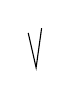
\begin{tikzpicture}[baseline=0cm,x=1cm,y=1cm]\draw[thin] (0,.32)--(.1,-.12)--(.17,.38);\end{tikzpicture}} $V\handwritten{\mapsto}V\otimes_{\underline{Q}_p}K$, and the \deleted{canonical} isomorphism between the restrictions is the obvious canonical isomorphism\inserted{\handwritten{(compatibility of $i$ with changes of base field)}}\handwritten{\begin{tikzpicture}[baseline=0cm,x=1cm,y=1cm]\draw[thin] (0,-.3)--(.04,.08)..controls (.3,.14) and (.45,.12)..(.6,.1)--(6.9,.12)..controls (7.1,.1) and (7.18,.18)..(7.2,.35);\end{tikzpicture}}. Thus the additional structure of $\underline{G}(k)$ (namely its canonical section \deleted{over} over $K$) is determined by the knowledge of the section of $\handwritten{\underline{\pi}}_p(k)$ over $K$ (i.e. the preceding functor $V\handwritten{\mapsto}V\otimes_{\underline{Q}_p}K$ ) and the isomorphism of the \unsure{iamge|image} of the said section in $\handwritten{\underline{\pi}}_p(\underline{F}_p)$ with the section coming from\deleted{\unsure{s}} the canonical section of $\handwritten{\underline{\pi}}_p(\underline{F}_p)$ over $\underline{Q}_p$ ; these are data which are obviously not contained in that of the group

\margin{\handwritten{\uline{NB} One thus has, by comparing the ``fibre ``\deleted{\unsure{forgetful}} at $\bar{k}$'' functor over $Q_p$, and the preceding functor, a canonical torsor over $K$ with group \deleted{\unsure{of}}\begin{tikzpicture}[baseline=0cm,x=1cm,y=1cm]\draw[gray,thin] (.12,.47)..controls (-.35,.31) and (-.26,-.35)..(.29,-.36);\end{tikzpicture}band $\underline{\pi}_p(k)_K$\deleted{\illegible{2} $\unsure{Q_p|\mathbb{Q}_p}$}}}
